\documentclass[a4paper,11pt]{article}


\usepackage{amsmath,amsfonts,amsthm,a4wide}
\usepackage{graphicx}
\usepackage[super]{nth}
\usepackage{mathtools}


\begin{document}
\begin{center}
University of Toronto at Scarborough\\[0.1in]
{\bf CSCC73H3 Algorithm Design and Analysis, FALL 2018} \\[0.1in]
{\large{\bf Assignment No.2: Greedy Algorithms}}\\[0.1in]
{\bf DUE:} September 29, 2018, at 11:59 pm
\end{center}


\vspace{0.1in}
\noindent
{\bf Student ID:} 1005642654 \\[0.15in]
{\bf Student Name:} KyooSik Lee
\vspace{0.3in}

\vspace{0.3in}
\begin{enumerate}

\item {\bf Description}

My greedy solution is the maximum spanning tree.

My greedy algorithm uses a slightly altered Kruskal's algorithm to give a greedy solution.
Kruskal's algorithm is originally designed for minimum spanning tree. 
My algorithm uses Kruskal's algorithm after multiplying -1 to each edge, which will result in maximum spanning tree.


{\bf Complexity}

Kruskal's algorithm first sort the edge by its weight.
The sorting takes $O(E\log{}E)$ time, where $E$ is the number of edges in the graph.



{\bf Correctness}

Follow the Kruskal's algorithm.

For any vertex $u$ and $v$, there is a moment in Kruskal's algorithm that by adding one edge makes $Set(u)$ = $Set(v)$(before adding $e$, $Set(u)\neq Set(v)$).
Let's call this edge $e$ with bandwidth $b_e$.
And let's call $p$ the greedy path at that moment from $u$ to $v$.
\begin{figure}[hbt]
	\centering
	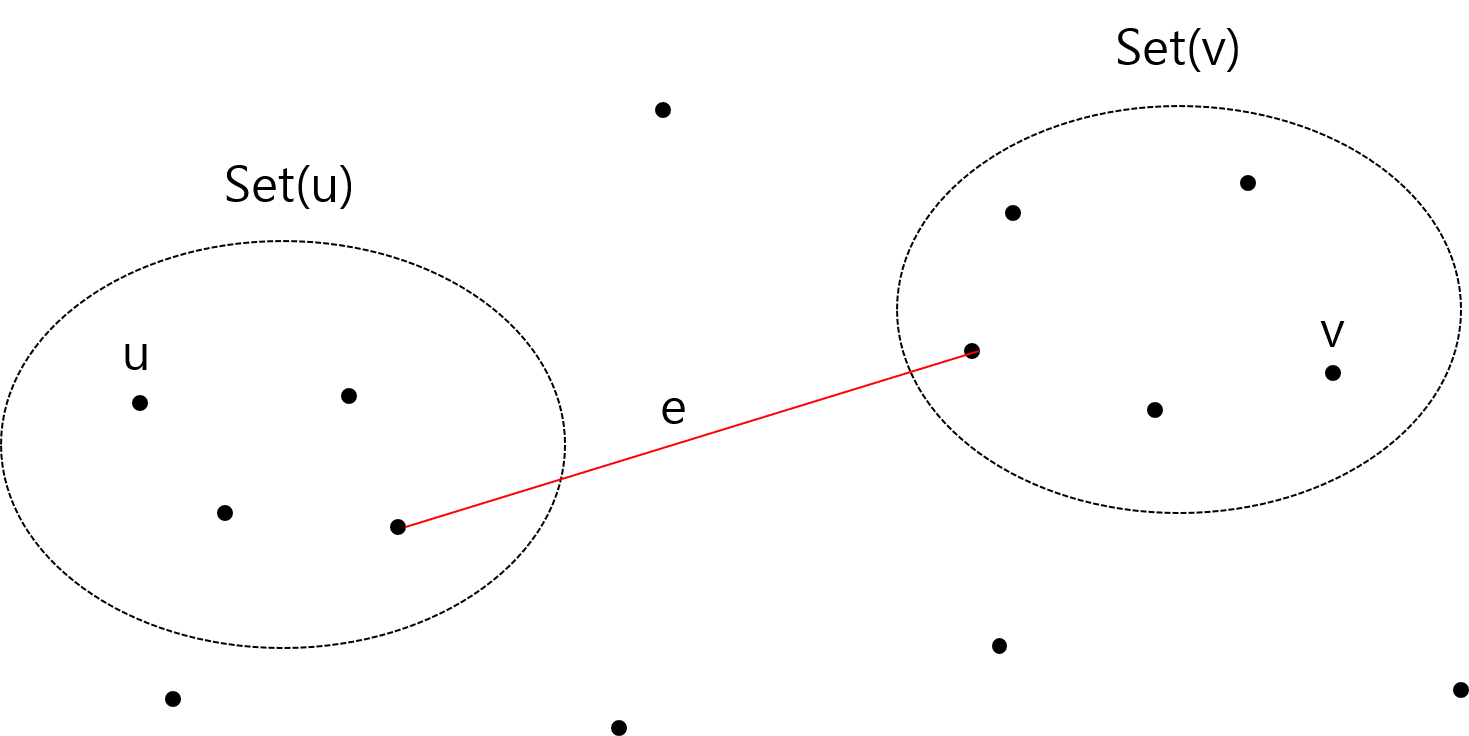
\includegraphics[scale=0.4]{figure1.png}
	\caption{Moment $e$ unions $Set(u)$ and $Set(v)$}
\end{figure}

By Kruskal's algorithm, any edge from the $set(u)$ to $set(v)$ other than $e$ has a smaller bandwidth than $b_e$.
Any path from $Set(u)$ to $Set(v)$ bypassing vertices/vertex outside of $Set(u)$ and $Set(v)$ will have smaller transmission bottleneck rate.
If not, unioning that vertices with either $Set(u)$ or $Set(v)$ must happen before $e$. 
If it happened before $e$ then adding $e$ to the maximum spanning tree will result in a cycle, which is a contradiction

For any vertex $u$ and $v$, by examing every direct path from $Set(u)$ to $Set(v)$ and bypassing path from $Set(u)$ to bypassing vertices/vertex to $Set(v)$ I have examined every possible path in the graph. 

Therefore, my greedy algorithm is correct. 




\item 

{\bf Description}

My greedy algorithm is to buy most profitable per dollar items first.

Profit per Cost $p_i$ is defined by $\frac{m_i-c_i}{c_i}$.
My algorithm is to buy largest $p_i$ items and moving on to next largest item until the budget is over.
The example table follows.


\begin{center}
\begin{tabular}{lcccc}
\bf{Item}               & A     & B                         & C    & D    \\
\bf{Cost/unit $c_i$}          & \$40  & \multicolumn{1}{c}{\$100} & \$20 & \$25 \\
\bf{MSRP} $m_i$               & \$100 & \$240                     & \$80 & \$75 \\
\bf{Available Quantity $q_i$} & 30    & 200                       & 500  & 200  \\
\bf{Profit per Cost $p_i$}  & \$1.5   & \$1.4                       & \$3    & \$2   
\end{tabular}
\end{center}

First look at the item that has largest $p_i$, and then buy as much as you can with your budget. If you still have budget left, look at the next item that has largest $p_i$. Repeat this until you have no budget left. If you have no more items to buy, terminate the algorithm.

{\bf Complexity}

First sorting the items according to its profit per cost takes $O(n\log{}n)$.

Then comparing each item to the budget will take $O(n)$ time.

Therefore, my algorithm's complexity is $O(n\log{}n)$.

{\bf Correctness}


Let's say we have an optimal solution O. 
Then O has better profit than our solution G.
For O and G lets sort each item bought according to it's profit so $p_1\geq p_2\geq \dots \geq p_n $, $p'_1\geq p'_2\geq \dots \geq p'_s $.
For money spent on O and G let's sort the money according to the profit each money makes. (Figure 2)

\begin{figure}[hbt]
	\centering
	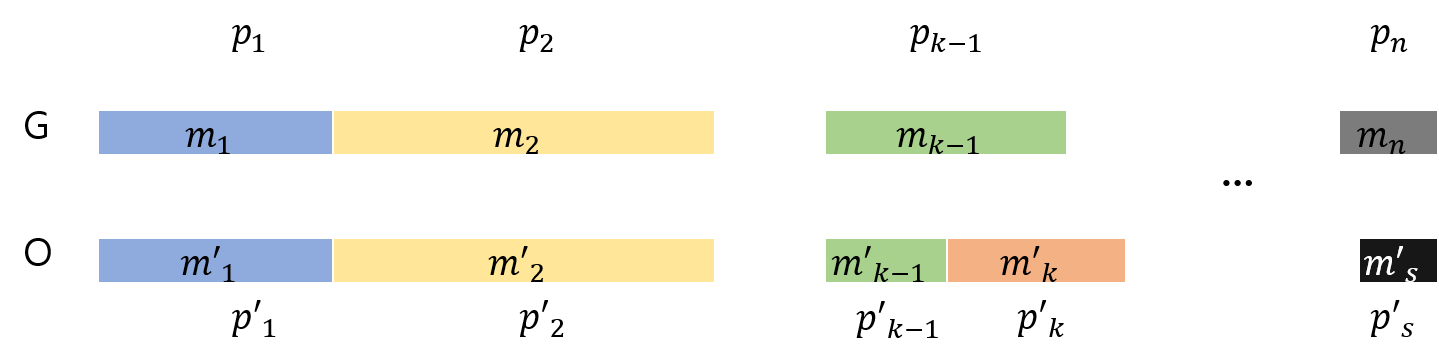
\includegraphics[scale=0.4]{figure2.png}
	\caption{Sorted Money According to Profit}
\end{figure}
Let's say $P(m)$ is the profit that money $m$ makes.
Then there exists $m'_k$ in O where $m'_{k-1} < m_{k-1} \& P(m'_k) \neq P(m_{k-1})$. Then for each money $m'_i (i\geq k)$, the profit $m'_i$ makes is less than the profit made by money above in the diagram. Then the total profit for $O$ is less than $G$, which is a contradiction to the fact that $O$ is optimal. 

Therefore my greedy algorithm is correct.

\end{enumerate}



\end{document}
